\documentclass[10pt,twocolumn,letterpaper]{article}

\usepackage{cvpr}
\usepackage{times}
\usepackage{epsfig}
\usepackage{graphicx}
\usepackage{amsmath}
\usepackage{amssymb}

% Include other packages here, before hyperref.

% If you comment hyperref and then uncomment it, you should delete
% egpaper.aux before re-running latex.  (Or just hit 'q' on the first latex
% run, let it finish, and you should be clear).
\usepackage[breaklinks=true,bookmarks=false]{hyperref}

\cvprfinalcopy % *** Uncomment this line for the final submission

\def\cvprPaperID{****} % *** Enter the CVPR Paper ID here
\def\httilde{\mbox{\tt\raisebox{-.5ex}{\symbol{126}}}}

% Pages are numbered in submission mode, and unnumbered in camera-ready
\ifcvprfinal\pagestyle{empty}\fi
%\setcounter{page}{4321}
\begin{document}

%%%%%%%%% TITLE
\title{Colorization}

\author{Vincent Billaut\\
Department of Statistics\\
Stanford University\\
{\tt\small vbillaut@stanford.edu}
% For a paper whose authors are all at the same institution,
% omit the following lines up until the closing ``}''.
% Additional authors and addresses can be added with ``\and'',
% just like the second author.
% To save space, use either the email address or home page, not both
\and
Matthieu de Rochemonteix\\
Department of Statistics\\
Stanford University\\
{\tt\small mderoche@stanford.edu}
\and
Marc Thibault\\
ICME\\
Stanford University\\
{\tt\small marcthib@stanford.edu}
}

\maketitle
%\thispagestyle{empty}

%%%%%%%%% ABSTRACT

% TODO for final report

%\begin{abstract}
%   
%\end{abstract}

%%%%%%%%% BODY TEXT
\section{Introduction}

The problem of colorization is one that comes quickly to mind when thinking about interesting challenges involving pictural data. Namely, the goal is to build a model that takes the greyscale version of an image (or even an actual "black and white" picture) and outputs its colorized version, as close to the original as possible (or at least realistic, if the original is not in colors).

One clear upside to this challenge is that any computer vision dataset, and even any image bank really, is a proper dataset for the colorization problem (the image itself is the model's expected output, and its greyscale version is the input to the model).

Classical approaches to this task, \eg \cite{cheng2015deep} and \cite{dahl2016tinyclouds}, aim at predicting an image as close as possible to the ground truth, and notably make use of a simple $L_2$ loss, which penalizes predictions that fall overall too far from the ground truth. As a consequence, the models trained following such methods usually tend to be very conservative, and to give desaturated, pale results.
On the contrary, authors of \cite{zhang2016colorful} take another angle and set their objective to be "\textit{plausible} colorization" (and not necessarily \textit{accurate}). One of their methods to validate their results was to set up a blind testing experiment where human subjects had to determine, between their prediction and the ground truth, which one seemed more realistic (and they achieved very good performance).

Our goal is to reproduce the approach of \cite{zhang2016colorful}, as we consider the implementation more challenging in the way the loss function and the prediction mechanism are designed, and the results more visually appealing.

If we reach satistfactory results in a timely manner, we will consider tackling the task of colorizing videos, which, in order to fully take advantage of the input format, will need to incorporate the notion of consistency between consecutive frames in a sequence.

\section{Problem statement}

\subsection{Datasets}

As previously stated, any dataset is proper for the colorization task, and we are currently working with subsets of both the SUN dataset \cite{xiao2010sun} and ImageNet \cite{russakovsky2015imagenet}.

More precisely, we are tackling a simplified version of our general task: correctly colorizing scenes that involve beaches and seashores. The idea behind this simplification is that restricting our model to rather consistent scenes, where we typically find the same patterns (the top of the scene is usually the sky, \ie blue, and the bottom usually sand, \ie yellow or brown, as shown by the example of Figure \ref{inex}), will enable us to have a working proof of concept, on top of which we can extend to bigger sets later. The "\texttt{beach\_sun}", "\texttt{coast}" and "\texttt{sandbar}" categories of the SUN database contain ??? pictures. The "\texttt{beach}", "\texttt{coast}" and "\texttt{seashore}" categories of ImageNet respectively contain 1713, 321 and 2382 pictures. This amounts to a total of (only) (?? = 4416+???) pictures, which doesn't appear to be much, but might be enough considering the reduction of our problem that we're focusing on.

\begin{figure}
\begin{center}
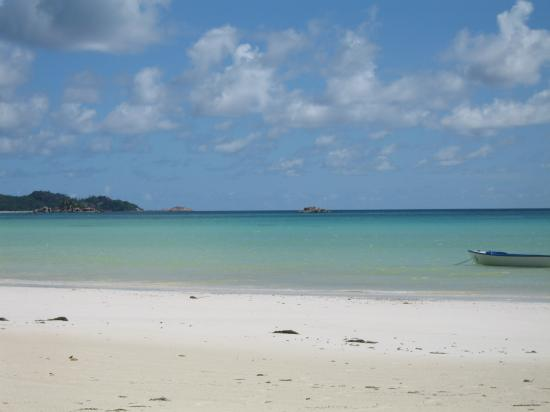
\includegraphics[width=200px]{img/beach.jpg}
\caption{Example of a picture from our reduced datasets (in this case, from \texttt{ImageNet/beach})}
\label{inex}
\end{center}
\end{figure}

Upon loading of an image, we switch the encoding from the RGB format to the YUV format, which means that the first dimension of every pixel encodes its grayscale value (the \textit{luminance}) and the two other encode the color itself (the \textit{chrominance}). This trick aims at simplifying the problem, because now the input is just one dimension of the image, and the expected output the two other dimensions.

\subsection{Expected results and evaluation}



\section{Technical approach}

\subsection{Overview}

% CNN approach
%	- classification, not regression
%	- prediction trick
%	- rebalancing trick
% considered GANs ?

The practical approaches to learning the color of a grayscale image can be split in two groups: the ones who take the angle of regression and try to predict a continuous color value, \eg \cite{cheng2015deep}, \cite{dahl2016tinyclouds} and \cite{deshpande2015learning}, and the ones who take an angle of classification, and discretize the color space into a finite amount of bins, \eg \cite{charpiat2008automatic} and \cite{zhang2016colorful}. Once again taking the angle of \cite{zhang2016colorful}, we're approaching the colorization as a classification problem.

Concretely, we want to discretize our colorspace, and for that we simply split our colormap into equal sized bins. As a first step, in order to reduce the computational toll, we don't want too many bins, and are therefore restricting our discretization to the $n$ most frequent color bins, as learned on a big dataset beforehand. In what follows, if a color from our actual image does not fall within one of our $n$ bins, we will simply assign it to the closest available. This simplification leads to a rather faint degradation of the images.

[exemple avec le bateau ???]

Following the approach of \cite{zhang2016colorful}, we want to boost the possibility of a rare color being predicted, and therefore reproduce the following tricks:
\begin{itemize}
\item Use \textit{rebalancing} to give larger weights to rare colors in our loss function. Precisely, each pixel value $p$, assigned to its closest bin $b \in \mathbb{R}^n$ is given a weight $w_p$ such that $$w_p \propto \left( (1-\lambda) \widehat{P}(b) + {\lambda \over n} \right)^{-1}$$ where $\widehat{P}(b)$ is the estimated probability of the bin (computed prior to our model's training).
\item Use an \textit{annealed-mean} to output predictions $y$ from the probability distribution $\textbf{Z}$ over our $n$ bins to the original, full color space. The idea is to find a compromise between taking the color class with the maximum probability (the mode), which gives a rather colorful result but sometimes lacking spatial consistency, and taking the weighted average over the bins, which gives a rather flat, sepia kind of tone. To achieve this we use a temperature parameter $T$ in the following softmax-like formula for one pixel $$y = f_T(\textbf{z}) = {\exp(\log(\textbf{z}) / T) \over \sum_i \exp(\log(\textbf{z}_i) / T)}$$ where $\textbf{z}$ is the $n$-dimensional probability vector of a given pixel over the $n$ bins, and the sum in the denominator is over all the bins. 
\end{itemize}

\begin{figure}
\begin{center}
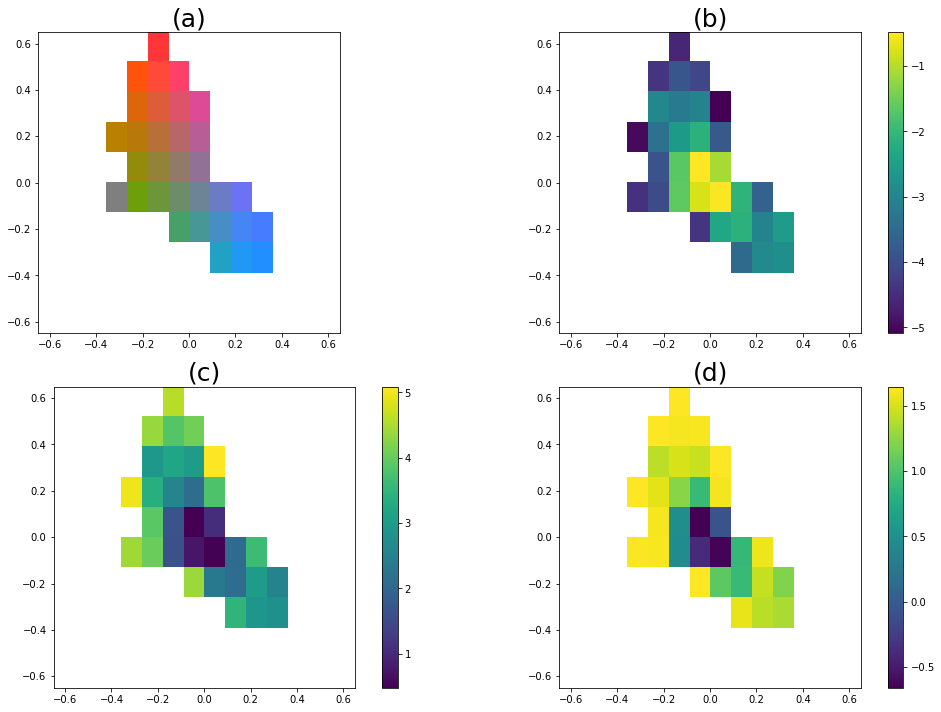
\includegraphics[width=250px]{img/cdexample.png}
\caption{(a) Color map, showing the mean color (\textit{chrominance}) of each of the selected bins (here, we set a threshold of 32 bins to select). (b) Frequency map (log-scale), shows the empirical frequency of the colors within each bin, computed over a dataset beforehand. (c) Inverse-frequency map (log-scale), \ie the inverse of (b). (d) Weight map (log-scale), shows the weights assigned to each bin after rebalancing. Interestingly, we notice that the amplitude in weights is much smaller than the amplitude in frequency (2 orders of magnitude against 4), which means that we partially make up for the underrepresentation bias and therefore encourage the prediction of rare colors.}
\label{cdex}
\end{center}
\end{figure}

Figure \ref{cdex} shows our discretized colorspace, as well as what the weights of the bins look like after rebalancing.



\subsection{Current model}

% details on 	# of layers
% 				sizes of layers
%				batch norm

\section{Preliminary results}

% our best hyper parameters yet
% one or two examples of predicted images

\section{Next steps}

{\small
\bibliographystyle{ieee}
\bibliography{references}
}

\end{document}
